\begin{abstract}
TODO
\end{abstract}

\chapter{Einleitung}
Schnelles 2D-Rendering ist eine nichttriviale Aufgabe für GPUs. Für viele Anwendungen sind die verfügbaren Bibliotheken im Allgemeinen immer noch viel zu langsam. Um das zu verbessern, haben wir mit \textit{BunnySuite} ein Framework entwickelt, mit dem gängige 2D-Grafik-Bibliotheken einem automatisierten Stresstest ausgesetzt werden können.\\
Mit dem \textit{BunnyMark}\footnote{https://github.com/openfl/openfl-samples/tree/master/demos/BunnyMark} gab es bereits eine Metrik zum Vergleich von Bibliotheken. Jedoch wurde hier nur die Anzahl der gerenderten Objekte (in diesem Fall Häschen, deshalb der Name) gemessen, bei denen noch 60 fps erreicht werden. Diese Zahl war nur schwer zu interpretieren und musste für ein ausführlicheres Ranking durch aussagekräftigere Metriken, bspw. \textit{Renderzeit pro Frame bei X Objekten} ersetzt werden. Auch findet diese Messung bei BunnyMark zu Demozwecken nur interaktiv statt: Häschen werden per Mausklick zur Szene hinzugefügt. Im entwickelten BunnySuite-Framework können solche Messungen automatisiert erfolgen. Die Tests für mehrere Frameworks werden automatisch nacheinander gestartet und das Ergebnis wird in einem Diagramm zusammengefasst. Das Framework ist leicht erweiterbar, so dass man es mit wenig Aufwand an neue Bibliotheken anpassen kann.\\
Das vollautomatisierte Test-Framework soll Entscheidern der Spieleentwicklung die Möglichkeit eines Rankings bieten, um die richtige Bibliothek für ihre Anforderungen zu finden. Des Weiteren sollen Entwickler von Bibliotheken das Framework nutzen können, um ihre eigene Engine zu testen und zu optimieren. Die Leistungen der Bibliotheken können so transparent verglichen werden, was den Wettbewerb zwischen den Bibliotheken stimulieren und Anreize setzen soll, stärker an der Performanz zu arbeiten. 

\chapter{Zeitplan und Aufgabenverteilung}
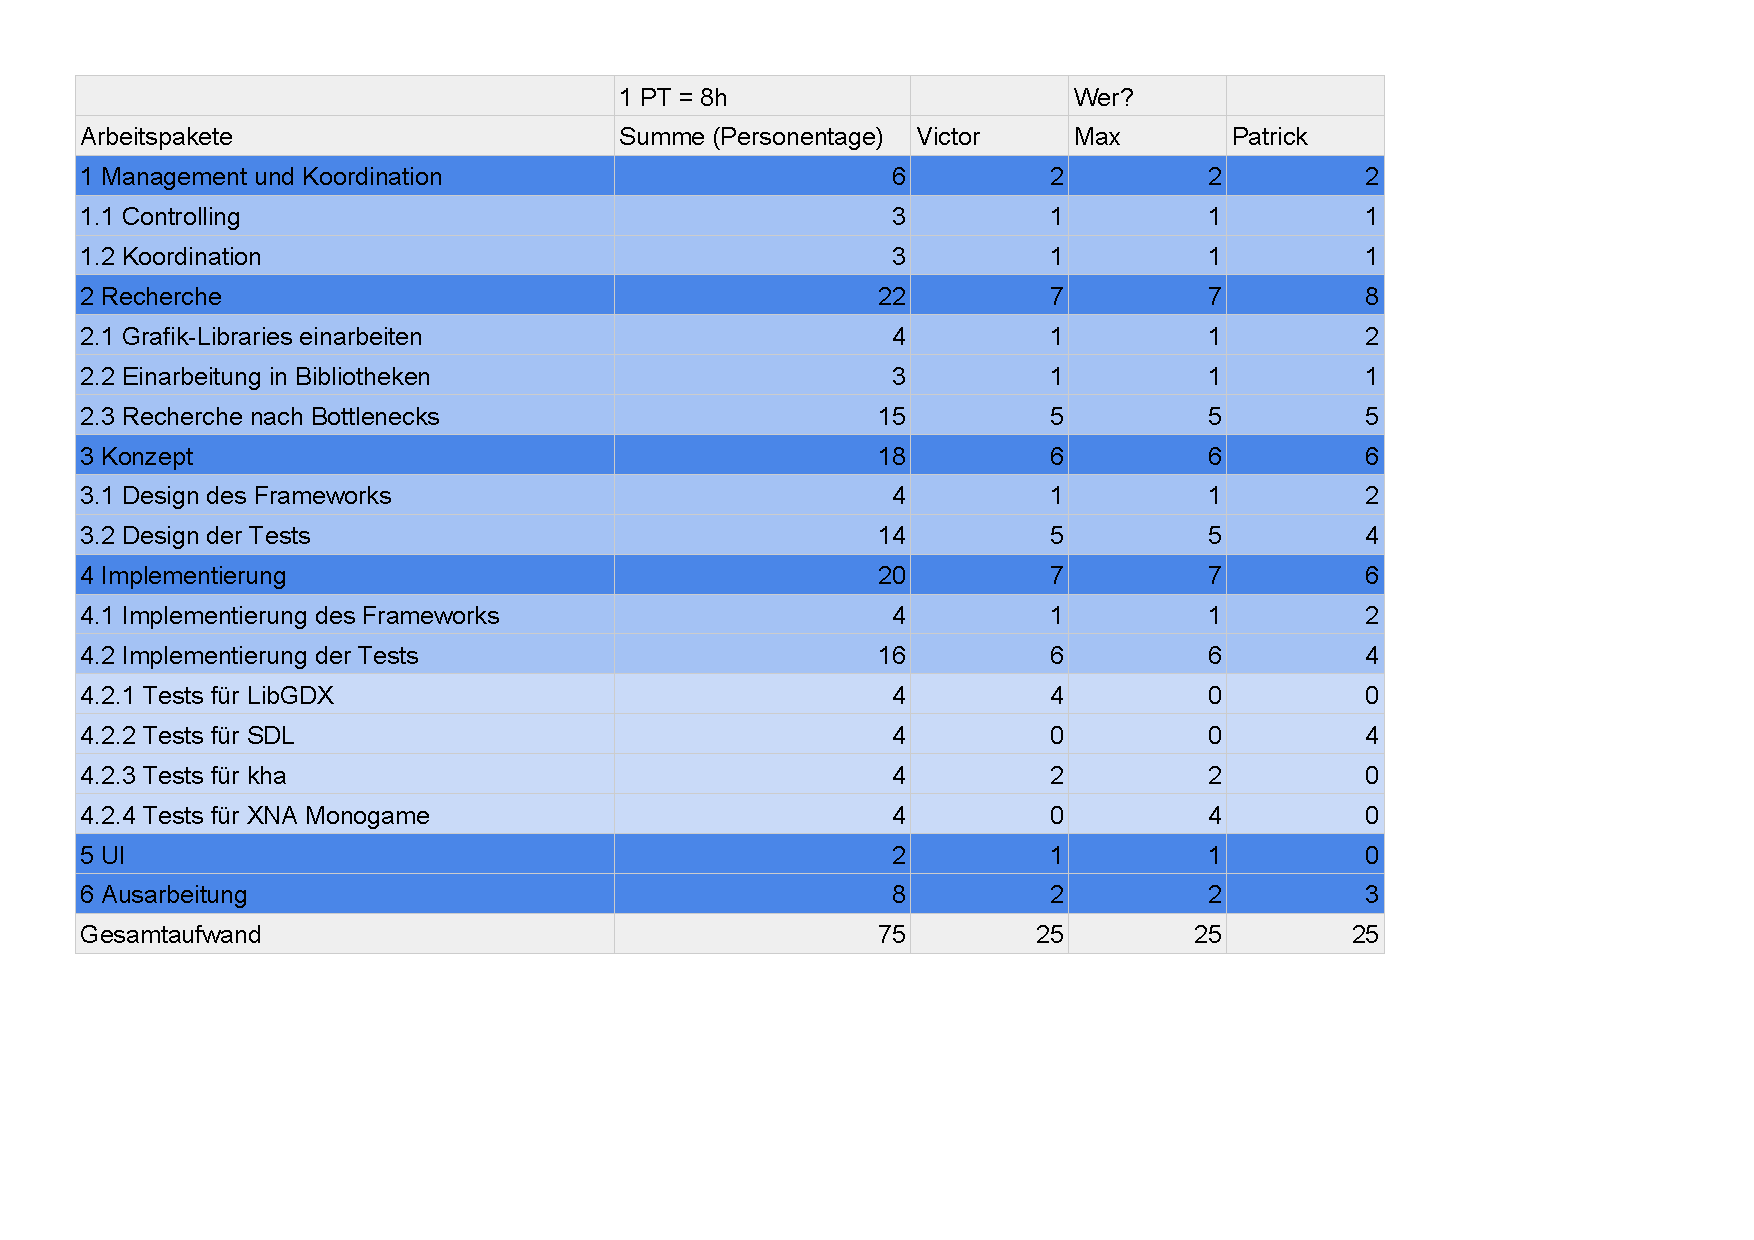
\includegraphics[width=1.2\textwidth]{projektplan.pdf}


\chapter{Grundlagen}
\section{2D-Frameworks}
\section{Benchmarking}
Der Benchmark soll vollautomatisiert erfolgen. Wichtigste Eigenschaft des Benchmarks ist die Vergleichbarkeit der Ergebnisse. Dazu wurde die Renderzeit pro Anzahl Bunnies als Kennzahl eingeführt. Wie bei allen empirischen Untersuchungen muss diese den folgenden drei Kriterien gen\"ugen:\\
\begin{itemize} 
\item \strong{Validit\"at}: Dass sich die Kennzahl mit empirischen Messergebnissen deckt ist garantiert, da sie empirisch zustande kommt. Es wurde die in Entwicklerkreisen \"ubliche Gr\"o\ss{}e {\em Renderzeit in Sekunden} gew\"ahlt, im Gegensatz zu ihrer Inversen, {\em Frames per Second}, oder einem arbitr\"aren Punktesystem. 
\item \strong{Objektivit\"at}: ist durch die Wohldefiniertheit der einzelnen Testverfahren gegeben (siehe \ref{sec:tests}).
\item \strong{Reliabilit\"at}: Als Ma\ss{}nahme f\"ur hohe Reliabilit\"at werden alle Messungen jeweils zehn mal durchgef\"uhrt und anschlie\ss{}end der Durchschnitt gebildet, um Einfl\"usse von Hintergrundprozessen zu minimieren. (siehe ..) 
% Falls es noch eine ausführliche Testreihe zur Reliabilität geben sollte, muss das hier noch eingefügt werden.
\end{itemize}

\chapter{Konzept und Design}
\section{Identifizierte Bottlenecks}
Da jede 2D-Grafik-Bibliothek ihre eigenen St\"arken und Schw\"achen aufweist und für unterschiedliche Zwecke optimiert ist, ist es wichtig, differenzierte Tests durchzuf\"uhren, um gezielt m\"ogliche Schwachstellen zu identifizieren, ohne dabei die St\"arken zu ignorieren. Zu diesem Zweck wurden verschiedene "Bottlenecks" identifiziert, also h\"aufige Schwachstellen, für die gezielt Tests entwickelt wurden. Diese sind unter anderem:\\
\begin{itemize} 
\item Animieren der Objekte
\item Objekte mit ver\"anderlichen Texturen
\item Vielzahl an gleichzeitig dargestellten Objekten mit unterschiedlichen Texturen
\item Skalierung der Objekte
\item Rotation der Objekte
\item Objekte mit (halb-)transparenten Texturen
\end{itemize}

\chapter{Umsetzung und Tests}
\section{Tests}
\label{sec:tests}

\chapter{Zusammenfassung und Ausblick}

